\documentclass{article}
\usepackage{listings}
\usepackage{color}
\usepackage{amsmath}
\usepackage{amsfonts}
\usepackage{amssymb}
\usepackage{caption}
\usepackage{polski}
\usepackage{indentfirst}
\usepackage{graphicx}
\usepackage{pdfpages}
\usepackage{gauss}

\DeclareCaptionType{equ}[][List of equations]
\captionsetup[equ]{labelformat=empty}

%script adding bars in matrix
\usepackage{etoolbox}
\makeatletter
\patchcmd\g@matrix
 {\vbox\bgroup}
 {\vbox\bgroup\normalbaselines}% restore the standard baselineskip
 {}{}
\makeatother

\newcommand{\BAR}{%
  \hspace{-\arraycolsep}%
  \strut\vrule % the `\vrule` is as high and deep as a strut
  \hspace{-\arraycolsep}%
}
\definecolor{dkgreen}{rgb}{0,0.6,0}
\definecolor{gray}{rgb}{0.5,0.5,0.5}
\definecolor{mauve}{rgb}{0.58,0,0.82}

\lstset{frame=tb,
  language=Python,
  aboveskip=3mm,
  belowskip=3mm,
  showstringspaces=false,
  columns=flexible,
  basicstyle={\small\ttfamily},
  numbers=none,
  numberstyle=\tiny\color{gray},
  keywordstyle=\color{blue},
  commentstyle=\color{dkgreen},
  stringstyle=\color{mauve},
  breaklines=true,
  breakatwhitespace=true,
  tabsize=3,
  extendedchars=\true,
  inputencoding=utf8x
}

\lstset{literate={ą}{{\k{a}}}1 {ł}{{\l{}}}1 {ń}{{\'n}}1 {ę}{{\k{e}}}1 {ś}{{\'s}}1 {ż}{{\.z}}1 {ó}{{\'o}}1 {ź}{{\'z}}1 {Ą}{{\k{A}}}1 {Ł}{{\L{}}}1 {Ń}{{\'N}}1 {Ę}{{\k{E}}}1 {Ś}{{\'S}}1 {Ż}{{\.Z}}1 {Ó}{{\'O}}1 {Ź}{{\'Z}}1 }

\begin{document}
\title{Sprawozdanie nr. 2 - Metody numeryczne i optymailzacja}
\author{Jakub Andryszczak 259519,\\ Jakub Żak 244255,\\ Maciej Cierpisz 249163}
\date{}
\maketitle

\newpage
\tableofcontents
%Tutaj zaczyna się wstęp

\newpage
\section{Zadanie nr. 1}

\section{Zadanie nr. 2}

Rozwiązać poniższy układ równań liniowych metodą eliminacji Gaussa z częściowym
wyborem element podstawowego:

\begin{lstlisting}

    import numpy as np

    A = np.array([ [4, 2, 0, 0],
                  [1, 4, 1, 0],
                  [0, 1, 4, 1],
                  [0, 0, 2, 4],])
    
    x = np.random.rand(4)
    print(x)
    print()
    
    def normal_power_method(A,x):
        for i in range(200):
         x = np.dot(A,x)
         x  = x/np.linalg.norm(x)
        
        return np.dot(np.dot(A,x),x)/np.dot(x, x)
    
    def shifted_power_method(A, x0, tol=1e-6):
      n = len(A)
      # Estimate a shift close to the smallest eigenvalue
      sigma = np.trace(A) / n
      x = x0.copy()
      for _ in range(200):
        y = np.dot(A, x) - sigma * x
    
      lambda_ = np.dot(x.T, np.dot(A, x))
      return lambda_
       
    
    lambda1 = normal_power_method(A, x) 
    lambda2 = 1 / normal_power_method(A, x)
    lambda3 = shifted_power_method(A, x)
    lambda4 = 1 / shifted_power_method(A, x)
    
    print("Largrest eigenvalue normal power",lambda1)
    print("Smallest eigenvalue normal power", lambda2)
    print("Largest eigenvalue shifted power", lambda3)
    print("Smallest eigenvalue shifted power", lambda4)
  
  \end{lstlisting}
  \newpage
  Poniżej wynik działania programu:
  \begin{figure}[h]
    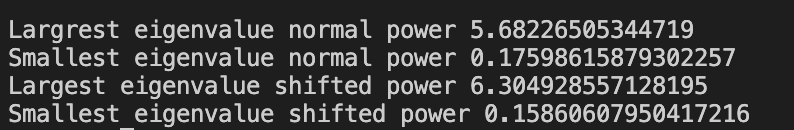
\includegraphics[scale=0.7]{image.png}
    \centering
    \caption*{Rys. 2 Wyniki obliczeń}
    \end{figure}

\section{Zadanie nr. 3}

\section{Zadanie nr. 4}

\section{Zadanie nr. 5}

\section{Zadanie nr. 6}

\section{Zadanie nr. 7}

\end{document} 